%% Validation of the phase-change (melting/solidification) implementation in PARTIES.
%% Format follows the JCP article template (elsarticle, review option).
\documentclass[review,12pt]{elsarticle}

\usepackage{amssymb}
\usepackage{amsmath}
\usepackage{float}
\usepackage{subcaption}
\usepackage{booktabs}
\usepackage{etoolbox}
\AtBeginEnvironment{tabular}{\def\baselinestretch{1}\selectfont}
\usepackage{lineno}

\journal{Journal of Computational Physics}

\newcommand{\uvec}{\mathbf{u}}
\newcommand{\Pet}{\mathrm{Pe}_T}
\newcommand{\Pes}{\mathrm{Pe}_S}
\newcommand{\Pech}{\mathrm{Pe}_{CH}}
\newcommand{\Ra}{\mathrm{Ra}}
\newcommand{\St}{\mathrm{St}}
\newcommand{\Nu}{\mathrm{Nu}}

\begin{document}

\begin{frontmatter}

\title{A diffuse-interface phase-change model for melting in salt-stratified
convection: implementation and validation in PARTIES}

\author[ucsb]{M. Jalabert}
\affiliation[ucsb]{organization={Department of Mechanical Engineering,
University of California Santa Barbara}, country={USA}}

\begin{abstract}
We present and validate a diffuse-interface melting model implemented in the
multiphase solver PARTIES. A conservative Cahn--Hilliard liquid fraction is
augmented with a superheat-driven Stefan source, coupled to a temperature
equation through a latent-heat sink that shares the same discrete field, so
that the discrete enthalpy $\int(\theta + F/\St)$ is conserved by construction.
Salt is confined to the liquid by a phase-weighted diffusivity, buoyancy uses a
quadratic (Roquet) equation of state, and the unmelted solid is held rigid by an
implicit Brinkman term that preserves the symmetric positive-definite structure
of the velocity solve. The implementation is verified against an exact
two-phase (binary) Stefan similarity solution, and validated against the melting
Rayleigh--B\'enard benchmark of Favier et al. and a flat-wall Rayleigh--B\'enard
Nusselt measurement. It is then applied to the salt-stratified lateral-melting
benchmark of Yang et al.\ (2023). We show that the apparent discrepancy with
that benchmark is dominated by a \emph{resolution-protocol} difference --- the
reference uses a dual-grid scheme in which velocity and temperature are carried
on a mesh five times coarser than the phase field, which a single-grid solver
cannot reproduce --- and that at matched effective resolution the freshwater
half-melt time and volume history agree to $4.7\%$ and $1.4\%$ respectively.
A residual $12.8\%$ difference in the salt-stratified melt rate is reported and
is shown \emph{not} to be a resolution artefact.
\end{abstract}

\begin{keyword}
phase change \sep Stefan problem \sep Cahn--Hilliard \sep diffuse interface \sep
double-diffusive convection \sep code validation
\end{keyword}

\end{frontmatter}

\linenumbers

\section{Introduction}
\label{sec:intro}

Melting of ice in contact with saline water couples a moving phase boundary to
double-diffusive convection with a nonlinear equation of state. Resolving this
coupling is a prerequisite for simulating sediment release from melting ice,
which motivates the present work.

This paper documents the phase-change extension of PARTIES and the evidence
supporting it. Section~\ref{sec:goveq} states the governing equations exactly as
solved; Section~\ref{sec:numerics} gives the discretisation, with attention to
the two properties that make the scheme usable --- discrete enthalpy
conservation and boundedness of the liquid fraction. Section~\ref{sec:validation}
verifies the implementation against an exact similarity solution and validates it
against two published benchmarks. Section~\ref{sec:yang} applies it to a
salt-stratified benchmark and analyses the comparison protocol, which turns out
to dominate the apparent agreement. Section~\ref{sec:limitations} states what
remains unresolved.

\section{Governing equations}
\label{sec:goveq}

The formulation is one-fluid and Boussinesq. The phase indicator $F$ is the
liquid (water) volume fraction, so the solid fraction is $\phi_s = 1-F$. Ice and
water share the reference density $\rho_0$, so the velocity field remains
solenoidal and no density jump enters the pressure projection. Lengths are
scaled by the domain height $H$, velocity by the free-fall scale
$U=\sqrt{g\,\Delta\rho\,H/\rho_0}$, temperature by
$\theta = (T-T_i)/\Delta T$ and salinity by $s = S/S_m$.

\subsection{Continuity and momentum}

\begin{equation}
  \nabla\cdot\uvec = 0 ,
  \label{eq:continuity}
\end{equation}
\begin{equation}
  \frac{\partial \uvec}{\partial t} + \nabla\cdot(\uvec\uvec)
  = -\nabla p
  + \sqrt{\frac{\mathrm{Pr}}{\Ra_T}}\,
    \nabla\cdot\!\left[\mu_r(F)\left(\nabla\uvec + \nabla\uvec^{\mathsf T}\right)\right]
  - b(\theta,s)\,\hat{\mathbf{y}}
  - \frac{\phi_s}{\tau}\,\uvec .
  \label{eq:momentum}
\end{equation}
The last term is a Darcy (Brinkman) penalisation active only inside the solid,
which holds the unmelted ice rigid. Its treatment is discussed in
Section~\ref{sec:brinkman}; $\sqrt{\mathrm{Pr}/\Ra_T} = 1/\mathrm{Re}$.

\subsection{Interface evolution}

The liquid fraction obeys a conservative Cahn--Hilliard equation with an added
melting source,
\begin{equation}
  \frac{\partial F}{\partial t} + \nabla\cdot(\uvec F)
  = \frac{1}{\Pech}\nabla^2\psi + m ,
  \qquad
  \psi = W'(F) - \mathrm{Cn}^2\nabla^2 F ,
  \label{eq:ch}
\end{equation}
with the double-well derivative
\begin{equation}
  W'(F) = \tfrac12 F(1-F)(1-2F) .
  \label{eq:doublewell}
\end{equation}
The mobility is constant. The Cahn number $\mathrm{Cn}$ sets the interface
thickness; the equilibrium profile is
$F = \tfrac12\left[1+\tanh\!\left(x/(2\sqrt{2}\,\mathrm{Cn})\right)\right]$,
whose $5$--$95\%$ thickness is $8.33\,\mathrm{Cn}$. No surface-tension force is
applied to the momentum equation: $\psi$ only regularises the interface.

\subsection{Stefan condition and liquidus}

The melting source is the superheat-driven phase-field form of Hester et al.,
\begin{equation}
  m = \frac{\St}{\Pet\,\epsilon}\,
      \bigl[\theta - \theta_L(s)\bigr]\, w(F),
  \qquad
  w(F) = \frac{F(1-F)}{\sqrt{2}\,\mathrm{Cn}},
  \qquad
  \theta_L(s) = T_m - \Lambda^{*} s ,
  \label{eq:melt}
\end{equation}
where $\epsilon$ is a band scale (taken equal to $\mathrm{Cn}$) and
$\St = c_p\Delta T/\mathcal{L}$. Note the convention: some authors define the
Stefan number inversely, $\St_{\mathrm{alt}} = \mathcal{L}/(c_p\Delta T) = 1/\St$.

The weight $w(F)$ equals $|\nabla F|$ on the equilibrium profile --- same
localisation, same unit integral --- but vanishes quadratically at the band
tails. This matters: the Cahn--Hilliard relaxation is much slower than the melt
deposition, so a source weighted by the measured $|\nabla F|$ keeps loading
nearly saturated cells and drives $F$ outside $[0,1]$, whereupon the
admissibility projection destroys melt mass for which the temperature field has
already paid latent heat. With $w(F)$ the deposition itself cannot push a cell
out of range.

The negative feedback between \eqref{eq:melt} and the latent sink below pins the
band temperature to the liquidus, so the interface superheat --- and with it the
front-speed error --- is $O(\epsilon)$. A one-sided flux-jump evaluation of the
Stefan condition is not usable on a diffuse band with nothing pinning the
interface temperature: the liquid- and solid-side gradients equalise and the
front stalls.

\subsection{Temperature and salinity}

\begin{equation}
  \frac{\partial \theta}{\partial t} + \nabla\cdot(\uvec\theta)
  = \frac{1}{\Pet}\nabla\cdot\!\left[\kappa_r(F)\nabla\theta\right]
  - \frac{1}{\St}\,m ,
  \label{eq:temperature}
\end{equation}
\begin{equation}
  \frac{\partial s}{\partial t} + \nabla\cdot(\uvec s)
  = \frac{1}{\Pes}\nabla\cdot\!\left(F\nabla s\right),
  \label{eq:salinity}
\end{equation}
with the phase-weighted diffusivity $\kappa_r(F) = \kappa_r^{\rm ice} +
(1-\kappa_r^{\rm ice})F$ evaluated at faces. Heat diffuses in both phases
($\kappa_r^{\rm ice}=1$ here); salt does not ($\kappa_r^{\rm ice}=0$), so
\eqref{eq:salinity} carries no salt flux into the ice. Meltwater dilution
therefore emerges from species conservation at the receding front rather than
from an explicit rejection source: $\int s\,\mathrm{d}V$ is conserved exactly,
and $s\equiv 0$ in the ice.

Crucially, the same discrete field $m$ appears in \eqref{eq:melt} and
\eqref{eq:temperature}, so the discrete enthalpy
\begin{equation}
  E = \int \left(\theta + \frac{F}{\St}\right)\mathrm{d}V
  \label{eq:enthalpy}
\end{equation}
changes only through boundary fluxes. This is the single most useful diagnostic
in the whole scheme and is monitored in every case below.

\subsection{Equation of state}

Buoyancy uses the quadratic (Roquet) equation of state, which places a density
maximum inside the temperature range and is essential to the cold-water dynamics:
\begin{equation}
  b(\theta,s) = -\beta_T\bigl|\theta - T_{md,0} - \sigma s\bigr|^{q}
                + \beta_S\, s ,
  \qquad q=2 .
  \label{eq:eos}
\end{equation}
The salinity-shifted density maximum is $\theta_{md}(s) = T_{md,0} + \sigma s$.
The slope $\sigma$ (a density-maximum shift) must not be confused with the
liquidus slope $\Lambda^{*}$ in \eqref{eq:melt}; they encode different physics.

\section{Numerical method}
\label{sec:numerics}

\subsection{Discretisation}

The solver uses a staggered MAC grid with second-order central differences for
momentum and scalars, and a fifth-order WENO scheme for the Cahn--Hilliard
advection $\nabla\cdot(\uvec F)$. Time advancement is a semi-implicit
low-storage three-stage Runge--Kutta scheme with coefficients
$\gamma = \{8/15,\,5/12,\,3/4\}$, $\zeta = \{0,\,-17/60,\,-5/12\}$ and
$\beta = \{4/15,\,1/15,\,1/6\}$: advective and source terms are explicit through
$\gamma,\zeta$, while viscous, diffusive, biharmonic and Brinkman terms are
implicit through $\beta$. The pressure Poisson equation is solved with HYPRE
(PCG preconditioned by PFMG); velocity and scalar Helmholtz systems use
preconditioned conjugate gradients.

\subsection{Cahn--Hilliard solve and the melt source}

The biharmonic operator is treated implicitly with coefficient
$\mathrm{Cn}^2/\Pech$. The melt source is evaluated pointwise from the
stage-lagged fields $F^{k-1}$ and $\theta^{k-1}$ before the liquid fraction is
updated, and rides the same $\gamma/\zeta$ combination as the advective and
diffusive terms. Being pointwise it needs no halo exchange and is exactly
rank-count independent.

\subsection{Boundedness and enthalpy conservation}
\label{sec:clip}

Conservative Cahn--Hilliard transport preserves $\int F$ but does not by itself
keep $F\in[0,1]$: the relaxation transient overshoots slightly behind an
advancing front. A per-stage projection restores admissibility, and the clipped
mass is redistributed back into the interfacial band with $F(1-F)$ weighting so
that the melt mass already paid for is not destroyed.

The magnitude of this correction is a diagnostic of whether the model is being
used inside its calibrated range. With the mapping $\mathrm{Cn} = 0.75\Delta x$
and $\Pech = 0.9/\mathrm{Cn}$ used throughout this paper, the cumulative clipped
mass reaches $2.4\%$ of the cumulative melt while the enthalpy drift stays at
$1.8\times 10^{-7}$ --- the correction is small and fully absorbed. Departing
from that mapping (for instance widening $\mathrm{Cn}$ at fixed mesh) breaks the
balance: the clip then handles $13\times$ the total melt and the enthalpy drift
rises to $8\times10^{-3}$, with a correspondingly meaningless melt rate. The
mapping is therefore a calibrated pair, not two free parameters, and enthalpy
drift should be checked before any melt rate is believed.

\subsection{Ice rigidity}
\label{sec:brinkman}

The Darcy term in \eqref{eq:momentum} is not an explicit source. It enters the
face-centred velocity Helmholtz solve as a positive local diagonal,
\begin{equation}
  \left[\frac{\rho_f}{\alpha_k \Delta t}
        + \frac{2\rho_f \phi_{s,f}}{\tau}\right]\uvec_f
  - \frac{1}{\mathrm{Re}}\nabla\cdot(\mu\nabla \uvec_f)
  = \mathrm{RHS} ,
  \label{eq:brinkman}
\end{equation}
so the operator stays symmetric positive-definite, the conjugate-gradient solver
and its Jacobi preconditioner are unchanged, and the pressure equation is
untouched. The associated boundary-layer thickness is
$\delta = \sqrt{\nu\tau}$, which for the parameters used here is a fraction of a
cell, so the penalised solid acts as an effective no-slip wall.

\section{Verification and validation}
\label{sec:validation}

\subsection{One-dimensional two-phase (binary) Stefan problem}
\label{sec:stefan}

The sharpest available test couples the Stefan condition, the liquidus and the
salt transport simultaneously, and has an exact solution. A planar interface
separates saline liquid from fresh ice; the melting temperature is depressed by
the local salinity. Self-similar solutions exist with the front at
$X(t) = X_0 + 2\lambda\sqrt{t/\Pet}$, where $\lambda$ solves
\begin{equation}
  \frac{\lambda\sqrt{\pi}\,e^{\lambda^2}}{\St}
  = \frac{\theta_\infty-\theta_i}{1+\mathrm{erf}\,\lambda}
  + \frac{\theta_{\rm ice}-\theta_i}{\mathrm{erfc}\,\lambda},
  \qquad
  s_i = \frac{s_\infty}
  {1+\sqrt{\pi}\lambda_s e^{\lambda_s^2}\left(1+\mathrm{erf}\,\lambda_s\right)},
  \label{eq:similarity}
\end{equation}
with $\lambda_s = \lambda\sqrt{\mathrm{Le}}$ and $\theta_i = -\Lambda^{*}s_i$.
Inputs are given in Table~\ref{tab:stefan-inputs}. For these parameters
\eqref{eq:similarity} gives $\lambda = 0.21713827$,
$s_i = 1.16402\times10^{-3}$ and $\theta_i = -5.82010\times10^{-4}$.

\begin{table}[H]
\centering
\caption{Inputs for the binary Stefan verification.}
\label{tab:stefan-inputs}
\begin{tabular}{l l}
\toprule
Parameter & Value \\
\midrule
Domain $L_x\times L_y$ & $1.5 \times 7.8125\times10^{-3}$ \\
Grid $N_x\times N_y\times N_z$ & $768\times 4\times 1$ \\
Initial interface $X_0$ & $0.75$ \\
Thermal P\'eclet $\Pet$ & $100$ \\
Solutal P\'eclet $\Pes$ & $10^4$ \\
Lewis number $\mathrm{Le}$ & $100$ \\
Stefan number $\St = c_p\Delta T/\mathcal{L}$ & $0.5$ \\
Liquidus slope $\Lambda^{*}$ & $0.5$ \\
Melting temperature $T_m$ & $0$ \\
Cahn number $\mathrm{Cn}$, band scale $\epsilon$ & $1.46484375\times10^{-3}$ \\
Cahn--Hilliard P\'eclet $\Pech$ & $614.4$ \\
Far-field $\theta_\infty$, $s_\infty$, ice $\theta_{\rm ice}$ & $1$, $1$, $0$ \\
End time & $0.5$ \\
\bottomrule
\end{tabular}
\end{table}

Figure~\ref{fig:stefan} compares the computed interface trajectory and the final
salinity profile against \eqref{eq:similarity}. The front follows the
$\sqrt{t}$ law from the first output, and the compositional boundary layer ---
only $\sqrt{t/\Pes}\approx 7\times10^{-3}$ thick, an order of magnitude thinner
than the thermal layer --- is captured without oscillation. Quantitative results
are in Table~\ref{tab:stefan-results}. The flow remains exactly quiescent
($\max|\uvec| = 0$), confirming that the melt source introduces no spurious
velocity.

\begin{figure}[H]
  \centering
  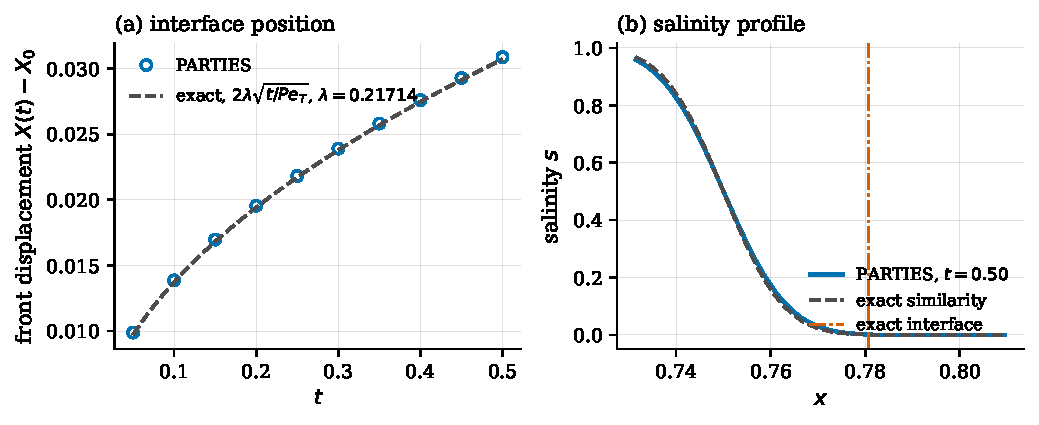
\includegraphics[width=\textwidth]{figures/stefan_binary.pdf}
  \caption{Binary Stefan verification at $\mathrm{Le}=100$. (a) Interface
  displacement against the exact similarity law
  $X(t)-X_0 = 2\lambda\sqrt{t/\Pet}$ with $\lambda = 0.21714$ from
  \eqref{eq:similarity}; symbols are simulation outputs. (b) Salinity profile at
  $t=0.5$ against the exact similarity profile, with the exact interface
  position marked. Salinity falls to $s_i\approx 1.2\times10^{-3}$ at the front
  because the released meltwater is fresh.}
  \label{fig:stefan}
\end{figure}

\begin{table}[H]
\centering
\caption{Binary Stefan verification: computed against exact.}
\label{tab:stefan-results}
\begin{tabular}{l r r r}
\toprule
Quantity & Computed & Exact & Relative error \\
\midrule
Similarity constant $\lambda$ & $0.2184496$ & $0.2171383$ & $6.0\times10^{-3}$ \\
Front-fit RMS residual & $6.3\times10^{-6}$ & --- & --- \\
Final liquid-salinity $L_\infty$ error & $1.44\times10^{-2}$ & --- & --- \\
Salt conservation drift & $6.0\times10^{-15}$ & $0$ & --- \\
Enthalpy drift & $5.0\times10^{-10}$ & $0$ & --- \\
Maximum velocity & $0$ & $0$ & --- \\
\bottomrule
\end{tabular}
\end{table}

\subsection{Melting Rayleigh--B\'enard convection}
\label{sec:meltingrb}

Convective melting is validated against the melting Rayleigh--B\'enard benchmark
of Favier, Purseed \& Duchemin, in which a solid layer melts from below into a
convecting fluid. Inputs are in Table~\ref{tab:meltingrb}. The benchmark has two
regimes: an early conduction-dominated phase in which
$(\tfrac12+\St_{\mathrm{alt}})\,\mathrm{Pe}\,\dot h$ takes a known constant
value, and a later convective plateau in which the effective Nusselt number
follows an $\Ra_e^{1/3}$ scaling.

\begin{table}[H]
\centering
\caption{Inputs for the melting Rayleigh--B\'enard validation.}
\label{tab:meltingrb}
\begin{tabular}{l l}
\toprule
Parameter & Value \\
\midrule
Domain $L_x\times L_y$ & $6 \times 1$ \\
Grid $N_x\times N_y\times N_z$ & $3072\times 512\times 1$ \\
Reynolds number $\mathrm{Re}=\sqrt{\Ra/\mathrm{Pr}}$ & $3162.28$ \\
Thermal P\'eclet $\Pet$ & $3162.28$ \\
Stefan number $\St = c_p\Delta T/\mathcal{L}$ & $10$ ($\St_{\mathrm{alt}}=0.1$) \\
Melting temperature $T_m$ & $0.05$ \\
Liquidus slope $\Lambda^{*}$ & $0$ (no salt) \\
Cahn number $\mathrm{Cn}$, band scale $\epsilon$ & $1.46484375\times10^{-3}$ \\
Cahn--Hilliard P\'eclet $\Pech$ & $614.4$ \\
Darcy time $\tau$ & $10^{-4}$ \\
Initial solid thickness & $0.05$ \\
End time & $120$ \\
\bottomrule
\end{tabular}
\end{table}

\paragraph{Correspondence with the reference cases.} The reference reports four
parameter sets (its table~1). Our runs match its \emph{case D}
($\Ra = 10^{7}$, aspect ratio $\lambda = 6$, $\theta_M = 0.05$, Stefan number
swept), differing only in being three times finer in $x$
($3072$ against $1024$ points). Case D underlies the reference's figures~7, 9
and~10, so those admit a direct comparison. Its figures~4 and~5, by contrast,
show \emph{case C} --- $\Ra = 10^{8}$, $\lambda = 8$, on $4096\times1024$ ---
a ten-fold higher Rayleigh number in a wider box. Comparisons with those two
figures below are therefore \emph{phenomenological}: we compare the sequence of
events and the interface--flow coupling, not matched parameters.

Figure~\ref{fig:meltingrb} shows the mean interface height and the boundary heat
fluxes. In the diffusive phase the measured
$(\tfrac12+\St_{\mathrm{alt}})\mathrm{Pe}\,\dot h = 23.34$ against the
analytical $23.14$, a $0.9\%$ agreement, and the maximum deviation from the
exact one-dimensional Stefan solution over that phase is $1.7\%$. In the
convective plateau the effective coefficient
$\gamma_{\rm eff} = \Nu/\Ra_e^{1/3}$ is $0.0983$ against the published $0.115$
(ratio $0.854$); the interface energy balance closes to $0.996$. The
$\St$-dependence of the melt rate is likewise reproduced: the measured ratio
$\dot h(\St_{\mathrm{alt}}{=}0.1)/\dot h(\St_{\mathrm{alt}}{=}1) = 3.01$ against
an expected $2.5$.

\begin{figure}[H]
  \centering
  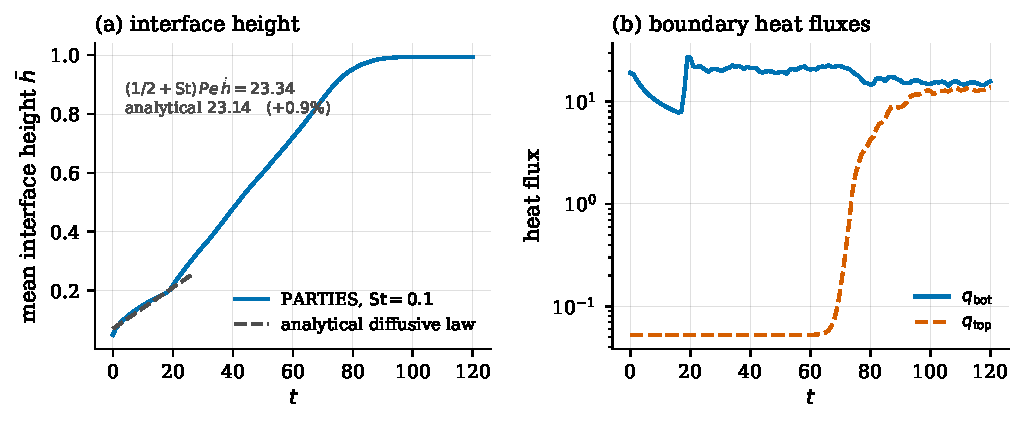
\includegraphics[width=\textwidth]{figures/melting_rb.pdf}
  \caption{Melting Rayleigh--B\'enard validation at $\St_{\mathrm{alt}}=0.1$,
  at the reference's case-D parameters. (a) Mean interface height, the quantity
  plotted in figure~7(a) of Favier et al.; the dashed line is the analytical
  diffusive-phase law, which the computation follows to $0.9\%$ before
  convection takes over near $t\approx20$. (b) Bottom and top boundary heat
  fluxes; the top flux rises by three orders of magnitude as the melt front
  reaches the upper boundary. The reference plots the bottom flux against depth
  in its figure~9, but only for $\St_{\mathrm{alt}}=10$.}
  \label{fig:meltingrb}
\end{figure}

\subsection{Melting Rayleigh--B\'enard: morphology and heat transport}
\label{sec:rbmorph}

Two further comparisons with Favier et al.\ test the model beyond the bulk melt
rate.

\paragraph{Melt-front topography.} Figure~\ref{fig:rbmorph}(a) shows the
interface position $h(x,t)$ at successive times, the diagnostic used in figure~7
of the reference. The front is flat while conduction dominates, develops cusps
once convection sets in near $t\approx20$, and coarsens as the layer deepens ---
each cusp sitting above the downwelling between two convection cells. At $t=70$
the interface carries $14$ extrema across $L_x=6$, a mean cusp spacing of
$0.86$, comparable to the fluid depth $h\approx0.78$ at that time and consistent
with one cusp per convective cell. Figure~\ref{fig:rbmorph}(b) shows the
corresponding temperature field with the melt front overlaid: the plumes and the
front topography are locked together, reproducing the qualitative behaviour of
the reference.

\begin{figure}[H]
  \centering
  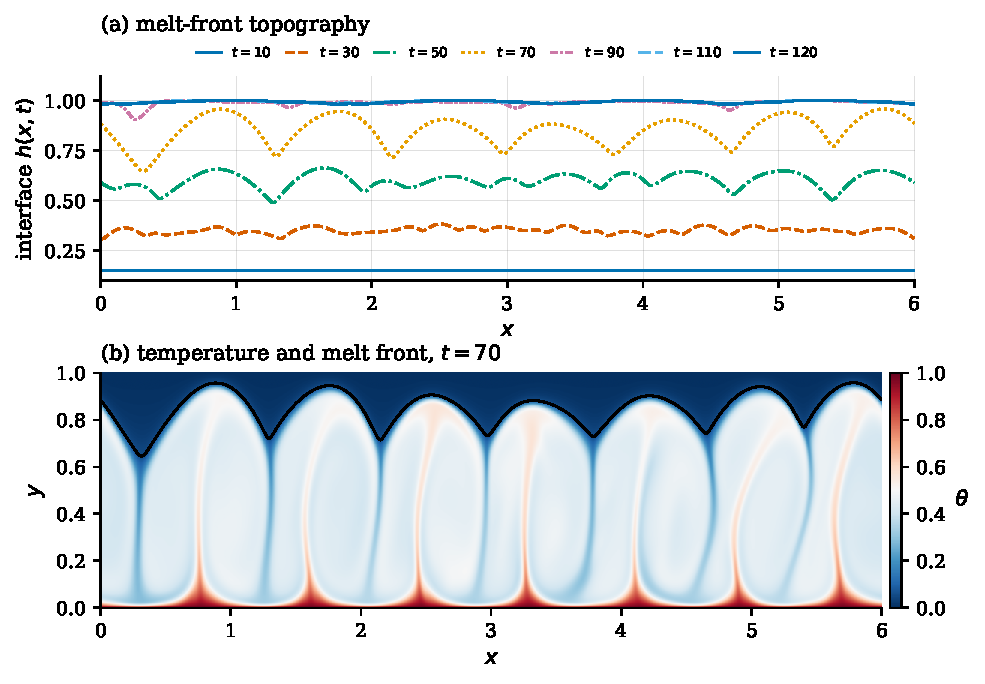
\includegraphics[width=\textwidth]{figures/rb_morphology.pdf}
  \caption{Melting Rayleigh--B\'enard at $\St_{\mathrm{alt}}=0.1$ (case-D
  parameters). (a) Interface position $h(x,t)$ at successive times: initially
  flat, cusped once convection begins, coarsening as the layer deepens.
  (b) Temperature field at $t=70$ with the $F=0.5$ melt front overlaid; each
  interface cusp sits above a downwelling. The corresponding diagnostics in
  Favier et al.\ are its figures~5(a) and~4, both computed for case C
  ($\Ra=10^8$, $\lambda=8$); the comparison here is phenomenological rather than
  parameter-matched, and the reference additionally colours its interface curves
  by signed curvature.}
  \label{fig:rbmorph}
\end{figure}

\paragraph{Full-domain evolution.} Figure~\ref{fig:rbpanels} reproduces the
six-panel visualisation of figure~4 of the reference: temperature on the left,
vorticity on the right, the $F=1/2$ interface overlaid, time increasing downward.
The sequence reproduces the reference's phenomenology in order. At $t=5$ the
layer is subcritical and motionless, the interface flat and the vorticity field
empty. By $t=20$ convection has set in at a short wavelength, and the front has
acquired matching small-scale cusps. Between $t=40$ and $t=80$ the cells grow
with the deepening layer and the wavelength coarsens, with cusps merging as
neighbouring cells combine. By $t=110$ the domain holds a few large counter-
rotating rolls whose downwellings sit under the remaining interface depressions.
The one-to-one correspondence between vorticity cells and interface cusps ---
the mechanism the reference identifies --- is visible at every stage.

\begin{figure}[H]
  \centering
  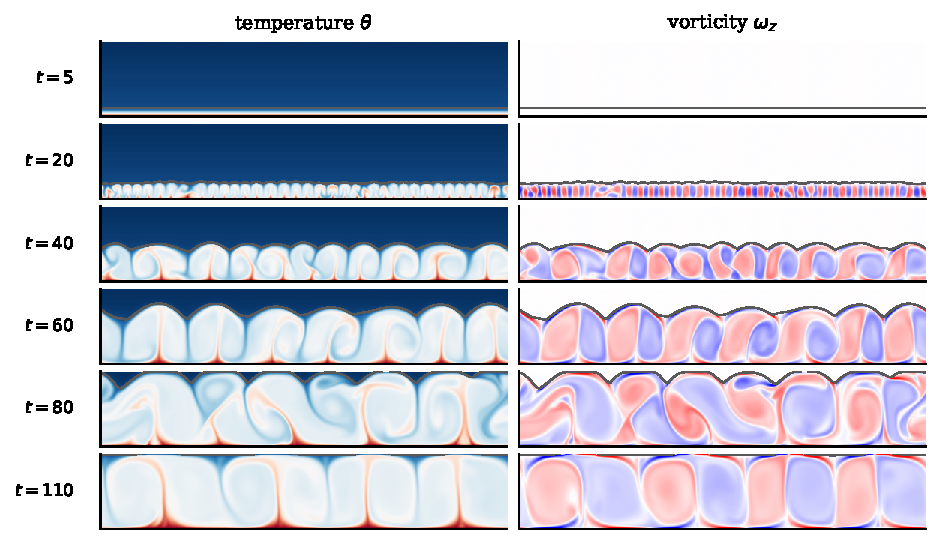
\includegraphics[width=\textwidth]{figures/rb_panels.pdf}
  \caption{Melting Rayleigh--B\'enard at $\St_{\mathrm{alt}}=0.1$ (case-D
  parameters): temperature (left, on the same scale as
  figure~\ref{fig:rbmorph}(b): dark blue $\theta=0$ to dark red $\theta=1$) and
  vorticity (right, $\pm0.25\,\omega_{\max}$) at six increasing times, with the
  $F=1/2$ interface in grey. Convection is absent at $t=5$, sets in at short
  wavelength by $t=20$, and coarsens as the fluid layer deepens; each interface
  cusp remains locked to a downwelling. Figure~4 of Favier et al.\ presents the
  same physics differently in two respects: it shows \emph{one} domain with
  temperature rendered over its left half and vorticity over its right half
  (the interface runs continuously across the join), and it is computed for case
  C ($\Ra=10^8$, $\lambda=8$) rather than case D. We show both fields over the
  whole domain instead, so that they can be read at the same location; the
  correspondence is in the sequence of events, not in the parameters.}
  \label{fig:rbpanels}
\end{figure}

\paragraph{Melting velocity against Stefan number.} The reference's figure~7(b)
gives the developed melting velocity as a function of Stefan number at case-D
parameters --- the same $\Ra$, aspect ratio and $\theta_M$ as our runs --- so our
two Stefan numbers fall directly on its curve. This is the one
DNS-to-DNS comparison available for this benchmark, and
Figure~\ref{fig:rbstefan} shows it: the computed melting velocities sit
$-4.8\%$ ($\St_{\mathrm{alt}}=0.1$) and $-15.3\%$ ($\St_{\mathrm{alt}}=1$) from
the reference values, on a quantity that varies by two orders of magnitude
across the plotted range.

\begin{figure}[H]
  \centering
  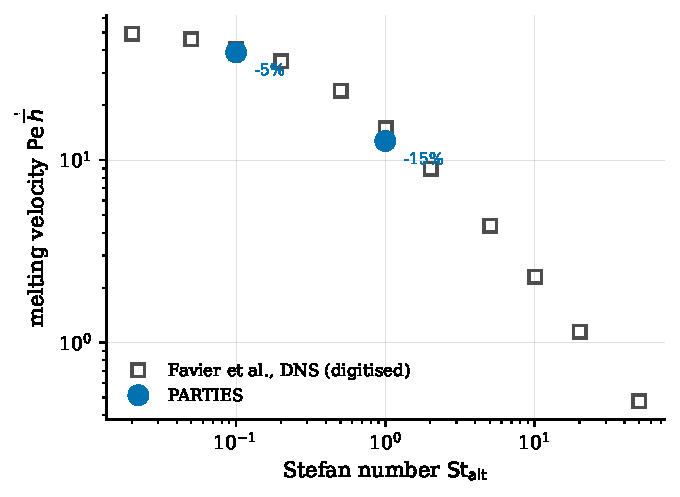
\includegraphics[width=0.62\textwidth]{figures/rb_stefan.pdf}
  \caption{Developed melting velocity against Stefan number, compared directly
  with the direct numerical simulations of Favier et al.\ (their figure~7(b),
  computed at the case-D parameters used here). Open symbols are their reported
  values, digitised from the published figure and re-plotted; filled symbols are
  the present computation, annotated with the relative difference.}
  \label{fig:rbstefan}
\end{figure}

\paragraph{Heat transport.} Figure~\ref{fig:rbheat} reproduces the
Nusselt--effective-Rayleigh relation of figure~10 of the reference, using
$\Nu = q_{\rm bot}h/(1-\theta_M)$ and $\Ra_e = \Ra(1-\theta_M)h^3$. Both melting
runs collapse onto a common $\Ra_e^{1/3}$ branch after the conduction plateau,
and the independently computed flat-wall point falls on the same branch --- which
is the substantive check, since it shows the melting interface is not perturbing
the heat transport law. The measured prefactor is
$\gamma_{\rm eff}=\Nu/\Ra_e^{1/3} = 0.093$ ($\St_{\mathrm{alt}}=0.1$) and
$0.097$ ($\St_{\mathrm{alt}}=1$), against $0.115$ in the reference: the scaling
exponent is reproduced, the prefactor sits $16$--$19\%$ low.

\begin{figure}[H]
  \centering
  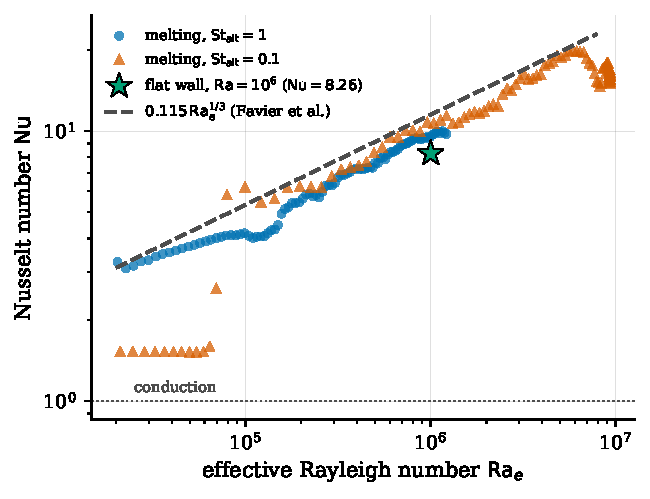
\includegraphics[width=0.72\textwidth]{figures/rb_heat_transport.pdf}
  \caption{Heat transport in the melting Rayleigh--B\'enard configuration
  (case-D parameters), the diagnostic of figure~10 of Favier et al. Both melting
  runs follow a common $\Ra_e^{1/3}$ branch once past the conduction plateau,
  and the independently computed flat-wall value lies on the same branch. The
  dashed line is the reference scaling $0.115\,\Ra_e^{1/3}$, which the reference
  measures at $\St_{\mathrm{alt}}=10$ --- an order of magnitude slower melting
  than either run shown here.}
  \label{fig:rbheat}
\end{figure}

\subsection{Flat-wall Rayleigh--B\'enard}

To separate convective transport from the phase-change model, the same solver
was run without melting in a flat-wall Rayleigh--B\'enard configuration at
$\Ra = 10^6$ on a $1024\times256$ grid. The measured Nusselt number over
$t\in[100,400]$ is $\Nu = 8.27\pm0.26$, with $\Nu_{\rm bot}$, $\Nu_{\rm top}$
and the volume-averaged value agreeing to $0.1\%$. This is at or slightly above
established correlations, confirming that the convective transport underlying
the melting cases carries no deficit.

\subsection{Single-physics gates}

Four additional one-dimensional gates were used during development to isolate
individual terms: a one-phase Stefan (Neumann) problem certifying the melt
source, latent sink and Stefan condition in isolation; a binary Stefan gate
certifying the liquidus coupling; a steady unidirectional-flow test that
reconstructs the buoyancy $b(\theta,s)$ of \eqref{eq:eos} pointwise from the
curvature of a velocity profile; and a Brinkman sweep measuring the Darcy
damping magnitude, its $\delta=\sqrt{\nu\tau}$ boundary layer and the
$\sqrt{\tau}$ slip scaling. All four passed. The raw outputs of these gates were
not retained, so they are reported here without figures; the binary Stefan case
of Section~\ref{sec:stefan} supersedes and strengthens the first two.

\section{Application benchmark: salt-stratified lateral melting}
\label{sec:yang}

\subsection{Configuration}

The benchmark of Yang et al.\ (2023) considers a vertical ice block of thickness
$0.1H$ melting laterally into stably salt-stratified water in a closed,
insulated square cavity. Inputs are given in Table~\ref{tab:yang-inputs}. Two
cases are used here: the freshwater case $S_m=0$ (which, having no salinity at
all, isolates thermally driven melting) and the salt-stratified reference case
$S_m = 5\,\mathrm{g\,kg^{-1}}$, $\Delta S_v = 5\,\mathrm{g\,kg^{-1}}$.

\begin{table}[H]
\centering
\caption{Inputs for the salt-stratified lateral-melting benchmark. Values marked
$\dagger$ are $S_m$-dependent and vanish in the freshwater case.}
\label{tab:yang-inputs}
\begin{tabular}{l l}
\toprule
Parameter & Value \\
\midrule
Domain, aspect ratio & $H\times H$, $\Gamma = 1$ \\
Initial ice thickness & $0.1H$, at $x\ge 0.9H$ \\
Thermal Rayleigh number $\Ra_T$ & $10^{7}$ \\
Prandtl number $\mathrm{Pr}$ & $10$ \\
Schmidt number $\mathrm{Sc}$ & $10^3$ ($\mathrm{Le}=100$) \\
Reynolds number $\mathrm{Re} = \sqrt{\Ra_T/\mathrm{Pr}}$ & $10^{3}$ \\
$\Pet$, $\Pes$ & $10^{4}$, $10^{6}$ \\
Stefan number $\St$ & $0.25$ ($\St_{\mathrm{alt}}=4$) \\
Liquidus slope $\Lambda^{*}$ $\dagger$ & $0.014$ \\
EOS $\beta_T$, $\beta_S$ $\dagger$, $T_{md,0}$, $\sigma$ $\dagger$
  & $1$, $1.75$, $0.2$, $-0.0625$ \\
Cahn number $\mathrm{Cn}$ & $0.75\,\Delta x$ \\
Cahn--Hilliard P\'eclet $\Pech$ & $0.9/\mathrm{Cn}$ \\
Darcy time $\tau$ & $10^{-4}$ \\
Boundary conditions & no-slip, no-flux on all walls \\
End time & $200$ \\
\bottomrule
\end{tabular}
\end{table}

\subsection{Resolution protocol}
\label{sec:protocol}

The reference simulations use a \emph{dual-grid} scheme: velocity and
temperature are carried on a base mesh of $288^2$, while salinity and the phase
field are refined five-fold to $1440^2$. PARTIES is single-grid, so no single
PARTIES run can match both simultaneously --- it is necessarily either
over-resolved in $(\uvec,\theta)$ or under-resolved in $(s,F)$ relative to the
reference. This is a structural difference in comparison protocol, not a
difference in the physical model, and it turns out to dominate the comparison.

Its consequence depends strongly on which case is considered. We therefore
measured the resolution dependence of both directly, over meshes from $216^2$ to
$1440^2$ (Table~\ref{tab:ladder}, Figure~\ref{fig:yang}a). Every run in the
ladder uses identical physical inputs and one binary; only the mesh and the four
mesh-tied numbers ($\mathrm{Cn}$, $\epsilon$, $\Pech$, $\Delta t$) vary.

\begin{table}[H]
\centering
\caption{Half-melt time $t_{1/2}$ as a function of mesh. The freshwater case is
strongly resolution-sensitive; the salt-stratified case is converged.}
\label{tab:ladder}
\begin{tabular}{l r r r r r r}
\toprule
$N$ & $216$ & $288$ & $360$ & $512$ & $720$ & $1440$ \\
\midrule
Freshwater $t_{1/2}$ & $116.31$ & $102.36$ & $94.47$ & $85.59$ & $78.89$ & $60.29$ \\
Salt-stratified $t_{1/2}$ & --- & $188.39$ & --- & $178.28$\rlap{$^{\ast}$} & --- & $179.85$\rlap{$^{\ddagger}$} \\
\bottomrule
\end{tabular}
\\[2pt]
\footnotesize $^{\ast}$ $N=432$. \quad
$^{\ddagger}$ Binary provenance unverifiable (Section~\ref{sec:limitations});
reported as corroborating only.
\end{table}

The freshwater half-melt time varies by $70\%$ across this range while the
salt-stratified one varies by $5.4\%$ and non-monotonically. The physical reason
is the benchmark's own mechanism: the vertical salinity gradient suppresses
convection, so the stratified flow is laminar enough to be resolved already at
$288^2$, whereas the freshwater case sustains vigorous convection whose heat
delivery is resolution-limited.

\subsection{Comparison at matched effective resolution}

Because the reference carries $(\uvec,\theta)$ on $288^2$ in both cases, and
because the freshwater case contains no salinity for the refined grid to act on,
the appropriate like-for-like comparison is PARTIES at $288^2$.
Table~\ref{tab:yang-results} and Figure~\ref{fig:yang}b give the result.

\begin{table}[H]
\centering
\caption{Comparison at matched effective resolution ($288^2$) and, for contrast,
at the finest mesh.}
\label{tab:yang-results}
\begin{tabular}{l r r r}
\toprule
Quantity & PARTIES $288^2$ & Reference & Difference \\
\midrule
Freshwater $t_{1/2}$ & $102.36$ & $107.42$ & $-4.7\%$ \\
Freshwater $V(200)/V_0$ & $0.2447\pm0.019$ & $0.2483$ & $-1.4\%$ \\
Salt-stratified $t_{1/2}$ & $188.39$ & $216\pm11$ & $-12.8\%$ \\
Melt-rate ratio $\bar f_5/\bar f_0$ & $0.543$ & $0.497$ & $+9.3\%$ \\
\midrule
\multicolumn{4}{l}{\emph{At $1440^2$ (protocol-mismatched):}} \\
Freshwater $t_{1/2}$ & $60.29$ & $107.42$ & $-43.9\%$ \\
Melt-rate ratio & $0.335$ & $0.497$ & $-32.6\%$ \\
\bottomrule
\end{tabular}
\end{table}

\begin{figure}[H]
  \centering
  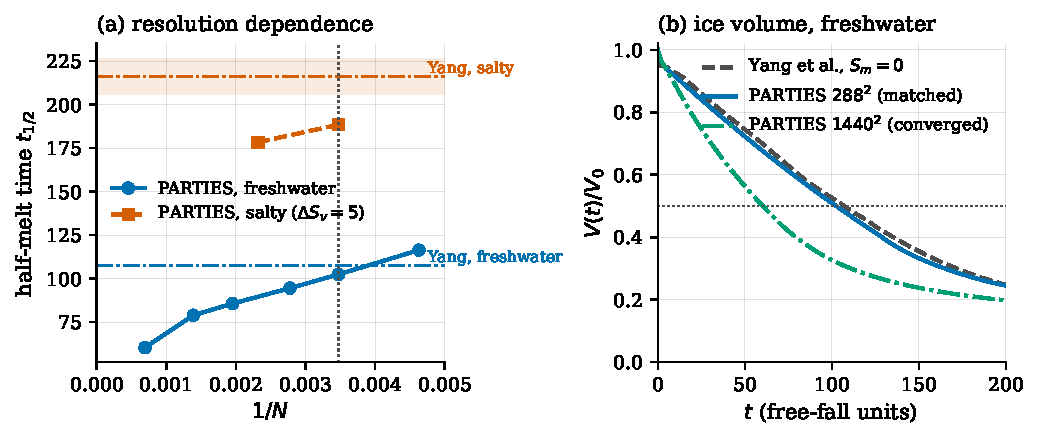
\includegraphics[width=\textwidth]{figures/yang_benchmark.pdf}
  \caption{Salt-stratified lateral-melting benchmark. (a) Half-melt time against
  inverse mesh size; horizontal lines are the reference values, the shaded band
  is the stated uncertainty of the salt-stratified reference, and the dotted
  vertical line marks the reference's $288^2$ base grid for velocity and
  temperature. The freshwater curve crosses its reference value at an effective
  $N=257$. (b) Freshwater ice-volume history: PARTIES at the matched $288^2$
  resolution tracks the reference closely, whereas the finer $1440^2$ run melts
  substantially faster.}
  \label{fig:yang}
\end{figure}

The freshwater curve crosses the reference value at an effective mesh of
$N = 257$, within $11\%$ of the reference's stated $288^2$ base grid. The
melt-rate ratio $\bar f_5/\bar f_0$ deserves particular note: it changes from
$-32.6\%$ to $+9.3\%$ purely by comparing at matched resolution, because its
numerator (freshwater) is resolution-sensitive while its denominator
(salt-stratified) is not, so a ratio formed at $1440^2$ is not commensurate with
one formed at $288^2$.

Melt-front morphology was also examined. The layered melt front predicted by
Huppert \& Turner has a spacing of $0.287H$ for these parameters; the computed
front gives $0.249$--$0.296H$ at $1440^2$ and $0.215$--$0.380H$ at $288^2$,
the latter with only three or four resolvable layers.

\subsection{Field structure and interfacial dynamics}
\label{sec:yangfields}

Beyond the integrated melt rate, two structural comparisons are available.

\paragraph{Layered fields.} Figure~\ref{fig:yangfields} shows temperature,
salinity and vertical velocity in the salt-stratified case. The stable salinity
gradient organises the flow into horizontal layers separated by sharp
interfaces, each layer carrying its own convective cell that impinges on the ice
--- the structure reported in figures~1 and~2 of the reference. Three layers are
present at this time, and the melt front is scalloped in phase with them.

\begin{figure}[H]
  \centering
  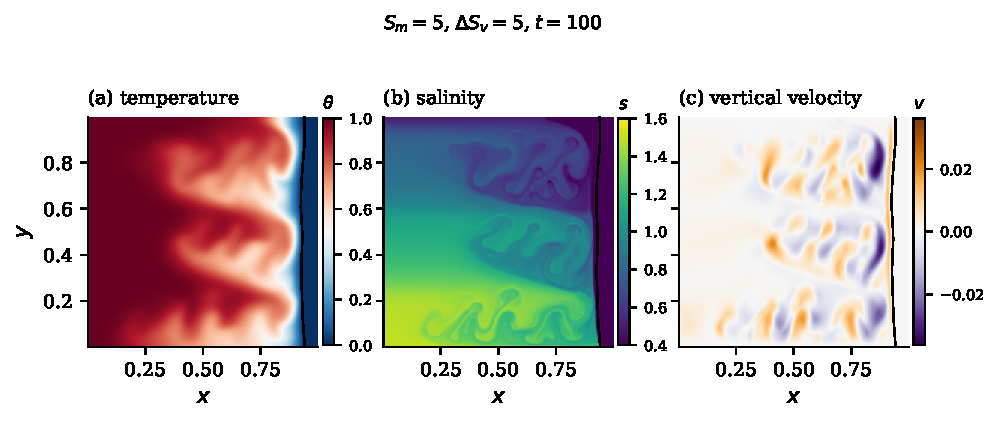
\includegraphics[width=\textwidth]{figures/yang_fields.pdf}
  \caption{Salt-stratified case at $t=100$: (a) temperature, (b) salinity,
  (c) vertical velocity, with the $F=0.5$ melt front overlaid in black. The
  stable salinity gradient organises the flow into three horizontal layers, each
  driving its own cell against the ice --- compare figures~1(c) and~2 of Yang et
  al. The vertical-velocity panel shows the circulation is confined within
  layers rather than spanning the cavity.}
  \label{fig:yangfields}
\end{figure}

\paragraph{Layer development in time.} Figure~\ref{fig:yangtimes} shows
temperature and salinity at four times, in the colour code of the reference
(temperature: \texttt{magma} over $\theta\in[0,1]$; salinity: \texttt{Blues}
over $s\in[0.5,1.5]$; solid masked white --- identified by matching their
published colourbars). The layers form early, at $t=40$, before a fifth of the
ice has melted, and persist while the front recedes: their number is set by the
imposed stratification rather than by the melt state.

\begin{figure}[H]
  \centering
  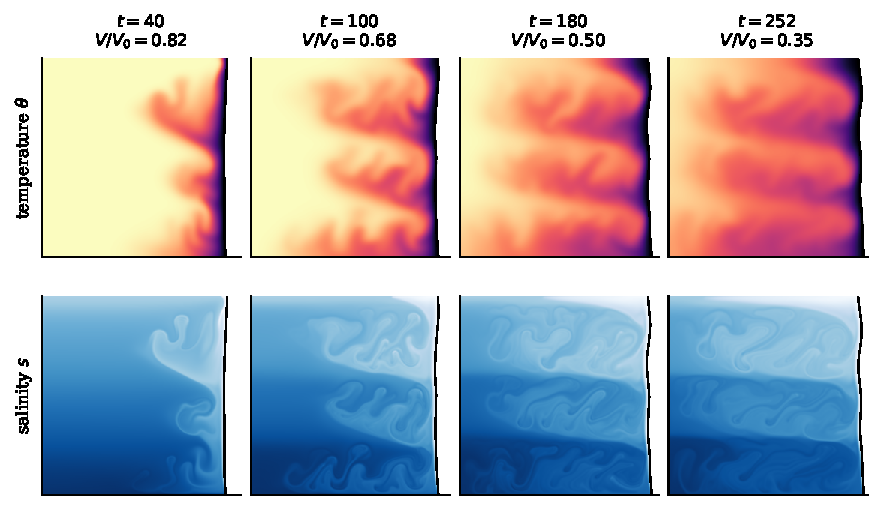
\includegraphics[width=\textwidth]{figures/yang_times.pdf}
  \caption{Temperature (top) and salinity (bottom) for the salt-stratified case
  at four times, in the colour code of Yang et al. Layers are established by
  $t=40$ and persist as the front recedes; the number of layers is set by the
  stratification, not by the amount of ice remaining.}
  \label{fig:yangtimes}
\end{figure}

\paragraph{Direct comparison of instantaneous fields.} Figure~\ref{fig:yangvs}
places our fields directly above the corresponding panel of figure~2(a) of the
reference, for the same case ($S_m=5$, $\Delta S_v=5$), in the same colour code
and with velocity vectors overlaid on the temperature field as they do.

The two are matched on \emph{melt state}, not on time, and the reason is worth
recording. The reference does not state the time of its figure-2 snapshots, and
it cannot be recovered reliably: locating each of its three $S_m=5$ panels on
the published volume curves by measuring the masked ice area gives mutually
inconsistent instants --- its $\Delta S_v=0$ panel corresponds to $t\approx191$,
whereas its $\Delta S_v=5$ panel holds $V/V_0=0.35$, a state that case cannot
reach by $t\approx191$ given its published half-melt time of $216$. The panels
are therefore evidently not a single synchronous set. We instead measured the
ice area in the reference panel, $V/V_0 = 0.35$, and show our field at the same
value, which occurs at $t=252$.

The structural agreement is close: both fields carry three well-defined layers
with sharp interfaces, both show the circulation confined within layers rather
than spanning the cavity, and both melt fronts are scalloped in phase with the
layering. Our field resolves finer filamentary structure within each layer,
consistent with the finer effective resolution discussed in
Section~\ref{sec:protocol}.

\begin{figure}[H]
  \centering
  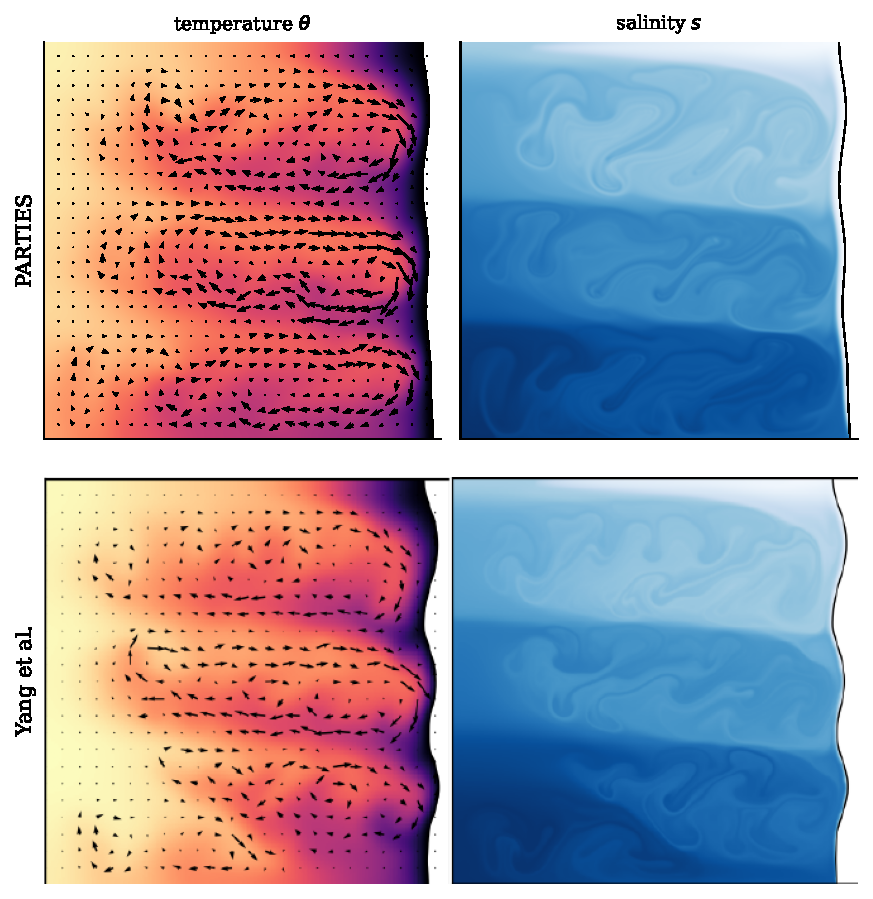
\includegraphics[width=0.86\textwidth]{figures/yang_vs_reference.pdf}
  \caption{Instantaneous temperature (left) and salinity (right) for
  $S_m=5$, $\Delta S_v=5$. Top: present computation at $t=252$. Bottom: the
  corresponding panel of figure~2(a) of Yang et al., reproduced under CC~BY~4.0.
  The two are matched at the same remaining ice fraction, $V/V_0=0.35$, because
  the reference does not publish the snapshot time (see text). Colour code and
  velocity-vector overlay follow the reference.}
  \label{fig:yangvs}
\end{figure}

\paragraph{Interfacial velocity and front shape.} Figure~\ref{fig:yangprof}(a)
reproduces the mid-height vertical-velocity profile of figure~4(b) of the
reference. In the freshwater case the cold, dense meltwater forms a strong
downward jet against the ice, peaking at $|v| = 0.080$ in free-fall units; the
reference reports a peak of $\approx0.085$ for its cases, so the magnitude of
the interfacial circulation is reproduced to within a few per cent. Adding
stratification weakens that jet by a factor of four, to $|v| = 0.021$, and
replaces it with a shallower oscillating profile --- the direct dynamical
expression of the suppression that makes the salt-stratified melt rate both
slower and resolution-insensitive (Section~\ref{sec:protocol}).

Figure~\ref{fig:yangprof}(b) contrasts the melt-front shapes. The freshwater
front is smooth and monotonic, with a peak-to-peak deviation from its mean tilt
of only $0.0056H$. The stratified front carries scallops of amplitude
$0.019H$, a factor $3.4$ larger, at the layer spacing.

\begin{figure}[H]
  \centering
  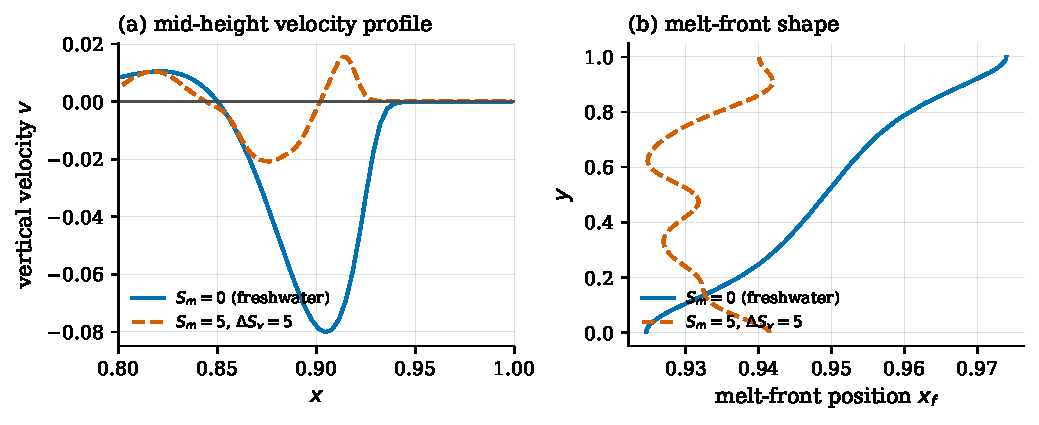
\includegraphics[width=\textwidth]{figures/yang_profiles.pdf}
  \caption{(a) Mid-height vertical-velocity profile at $t=100$, to be compared
  with figure~4(b) of Yang et al. The freshwater downward jet peaks at
  $|v|=0.080$ against a reported $\approx0.085$; stratification weakens it
  fourfold. (b) Melt-front position: smooth in freshwater, scalloped at the
  layer spacing when stratified.}
  \label{fig:yangprof}
\end{figure}

\paragraph{Front evolution and the density structure.}
Figure~\ref{fig:yangevol}(a) tracks the melt front through the run. The front is
nearly straight at $t=20$, and scallops emerge and deepen as the layers organise,
reaching an amplitude of $0.019H$ by $t=100$ while the mean position recedes.
Figure~\ref{fig:yangevol}(b) shows mid-height profiles of $\theta$, $s$ and the
buoyancy $b(\theta,s)$ of \eqref{eq:eos}, the diagnostic used in the inset of
figure~4(b) of the reference. Both scalars fall to their interfacial values over
the same narrow region, and $b$ follows the salinity rather than the temperature
--- with $\beta_S = 1.75$ against $\beta_T = 1$, and with the temperature anomaly
entering quadratically about the density maximum, the salinity term dominates the
buoyancy everywhere outside the immediate interfacial layer. This is the
mechanism behind the non-monotonic dependence of melt rate on mean salinity that
the reference reports, and it is what makes the freshwater and salt-stratified
cases behave so differently under mesh refinement
(Section~\ref{sec:protocol}).

\begin{figure}[H]
  \centering
  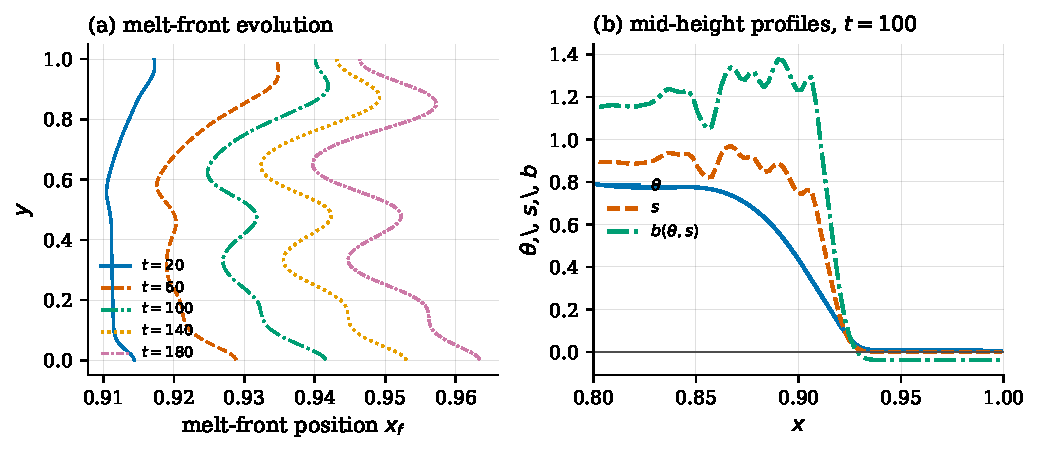
\includegraphics[width=\textwidth]{figures/yang_evolution.pdf}
  \caption{Salt-stratified case. (a) Melt-front position at successive times:
  initially straight, developing scallops at the layer spacing as the
  stratification organises. (b) Mid-height profiles of temperature, salinity and
  buoyancy at $t=100$, to be compared with the inset of figure~4(b) of Yang et
  al.; buoyancy tracks salinity rather than temperature outside the interfacial
  layer.}
  \label{fig:yangevol}
\end{figure}

\subsection{Summary of the comparison}

Table~\ref{tab:yang-qual} collects the structural comparisons alongside the
integrated ones of Table~\ref{tab:yang-results}.

\begin{table}[H]
\centering
\caption{Structural comparison with the reference. Quantities without a
published numerical value are marked as qualitative.}
\label{tab:yang-qual}
\begin{tabular}{l l l}
\toprule
Quantity & This work & Reference \\
\midrule
Peak mid-height $|v|$, freshwater & $0.080$ & $\approx0.085$ \\
Peak mid-height $|v|$, stratified & $0.021$ & --- (weakened, qualitative) \\
Layers in the stratified cavity & $3$ & $3$--$4$ (qualitative) \\
Melt-front amplitude, freshwater & $0.0056H$ & smooth (qualitative) \\
Melt-front amplitude, stratified & $0.019H$ & scalloped (qualitative) \\
Layer spacing & $0.215$--$0.380H$ & $0.287H$ (Huppert \& Turner) \\
Buoyancy dominated by & salinity & salinity \\
\bottomrule
\end{tabular}
\end{table}

\section*{Note on reproduced data}

Figure~\ref{fig:rbstefan} and the reference curves in
Figure~\ref{fig:yang}(b) re-plot values extracted from published figures of
Favier et al.\ (J.~Fluid Mech.\ \textbf{858}, 437--473, 2019) and Yang et al.\
(J.~Fluid Mech.\ \textbf{969}, R2, 2023) respectively. From Favier et al.\ only numerical values are reused and no figure image is
reproduced. Figure~\ref{fig:yangvs} does reproduce one panel of figure~2(a) of
Yang et al., which is permitted: that work is distributed under CC~BY~4.0, and
it is attributed in the caption. The Yang et al.\
preprint is distributed under CC~BY~4.0; the Favier et al.\ preprint carries the
arXiv perpetual non-exclusive licence, which does not grant third-party reuse of
the figures themselves, so reproducing any of its panels here would require
permission from the authors and the publisher.

\section{Limitations}
\label{sec:limitations}

We state the following explicitly rather than leaving them to inference.

\paragraph{Residual salt-stratified discrepancy.} The $-12.8\%$ difference in
the salt-stratified half-melt time is \emph{not} explained by the resolution
protocol, because that case is resolution-converged
(Table~\ref{tab:ladder}). It is $2.6\sigma$ against a reference value that is
itself derived --- obtained as the freshwater half-melt time divided by a
normalised melt rate read from a figure, and therefore carrying $\pm4.9\%$,
against $\pm2.8\%$ for the directly digitised freshwater targets. The
discrepancy is real and unexplained.

\paragraph{Mechanism versus number.} At $288^2$ the PARTIES diffuse band is
$5.3\times$ wider than the reference's phase-field interface ($2.17\times10^{-2}$
against $4.09\times10^{-3}$ in $5$--$95\%$ terms), although at $1440^2$ the two
agree to $6\%$. Both codes therefore under-deliver interfacial heat at the
matched effective resolution, plausibly for different reasons, and the agreement
in Table~\ref{tab:yang-results} may be numerically correct but mechanistically
coincidental. The experiment designed to separate mesh resolution from interface
width failed on the enthalpy-conservation criterion of Section~\ref{sec:clip} and
has not been repeated.

\paragraph{Band-localised corrections are ineffective.} A model refinement that
evaluates the liquidus and the equation of state on the liquid salinity
$s/(F+\delta)$ rather than the volume-averaged $s$ improves the similarity-solution
front constant by a factor $3.7$ in one dimension, but changes the
salt-stratified half-melt time by only $-0.09$ against the $+37.8$ that would be
required. The reason is that the Brinkman drag $\rho(2/\tau)\phi_s$ overlaps the
diffuse band, damping the velocity exactly where such a correction acts. Since
the reference's penalty is of comparable strength, this constrains both codes and
retires the whole family of band-localised corrections.

\paragraph{Late-time enthalpy drift.} The enthalpy drift is
$2.0\times10^{-5}$ at the freshwater half-melt point but grows to
$1.7\times10^{-3}$ by $t=200$, once the melt front reaches the far wall. Through
\eqref{eq:enthalpy} that bounds the accuracy of $V(200)/V_0$ at $\pm0.019$, so
the $-1.4\%$ agreement in Table~\ref{tab:yang-results} should be read as
consistency rather than as a $1.4\%$ measurement. The half-melt time is
unaffected.

\paragraph{Provenance.} The binary that produced the salt-stratified $1440^2$
run has been overwritten and its output is no longer accessible, so its
equivalence to the binary used for the ladder cannot be tested. That value is
therefore reported as corroborating only; no claim in this paper depends on it.

\section{Conclusions}

The phase-change implementation reproduces an exact two-phase Stefan similarity
solution to $0.6\%$ in the front constant with machine-precision salt
conservation and negligible enthalpy drift, reproduces the diffusive phase of a
published melting Rayleigh--B\'enard benchmark to $0.9\%$, and carries no
convective-transport deficit. Applied to a salt-stratified lateral-melting
benchmark, it reproduces the freshwater half-melt time to $4.7\%$ and volume
history to within its own systematic uncertainty when compared at matched
effective resolution, and reproduces the melt-rate ratio to $9.3\%$. A
$12.8\%$ residual in the salt-stratified melt rate is reported as unexplained.

The broader methodological point is that the apparent size of the discrepancy
depends almost entirely on the comparison protocol: the same data compared at
mismatched resolution give $-43.9\%$ and $-32.6\%$ where matched comparison
gives $-4.7\%$ and $+9.3\%$. Where a reference uses a multi-resolution scheme
that a single-grid solver cannot reproduce, the resolution dependence of each
code must be measured before any difference between them is attributed to the
physical model.

\end{document}
